\chapter{GEOMETRY:\\ INQUIRY-BASED APPROACH}
\section*{INTRODUCTION}
This module presents Inquiry-Based Learning (IBL) as an alternative teaching strategy in
introducing geometry. The first part of the model will let the participants experience an inquiry-
based activity. After which, the activity will be examined on how it was implemented. From the
discussion, definition as well as some models of inquiry-based learning will be discussed. In the
afternoon, participants will have to develop their own lesson plan, activity or worksheet using
inquiry-based learning. Outputs will then be presented for comments and critiquing. Aside from
the models, sample activities, lesson plans, and assessment will also be included.
\section*{OBJECTIVES}
After completing this module, you should be able to:
\begin{enumerate}
\item Experience inquiry-based lesson.
\item Define Inquiry-Based Learning including its factors and essential elements.
\item Identify different models for Inquiry-Based Learning.
\item Develop inquiry-based activity sheets for geometry.
\end{enumerate}
\section*{MATERIALS}
\begin{tabular}{lll}
LCD Projectors & Manila Papers & White Board Markers\\
Permanent Markers & Colored and White Chalks & Bond Markers\\
\end{tabular}

\underline{For Group Activity 1 ( 1 set per group of 5 or 6 participants)}

\begin{tabular}{llll}
Manipulatives & Pencils & Ruler/Meter Stick & Permanent Marker\\
Manila Paper & Crayons & Masking tape & \\
\end{tabular}

\underline{For Group Activity 2 ( 1 set per group of 5 or 6 participants)}

\begin{tabular}{lll}
Manila Paper & Permanent Marker & Masking Tape \\
\end{tabular}

\section*{GROUP ACTIVITY 1}
Participants are to be divided into groups of 5 or 6. This can be done through ice
breakers such as “The Boat is Sinking...” or other games (You may also refer to the site
\url{http://www.girlscoutsnorcal.org/documents/LE-Fun_Splitters.pdf}).

After the groups have settled down and formed a circle, each group will be given an
envelope containing the set of manipulatives with the instructions and guide questions. One set
of manipulatives contains the following figures: square, rectangle, rhombus, parallelogram,
trapezoid, isosceles trapezoid, and kite. Figures may be of different sizes. Answers and outputs
will be written/drawn on a manila paper.

\subsection*{PROCEDURE}

\begin{enumerate}
\item Open the envelope and place the contents on the table/floor.
Guide Questions:
	\begin{enumerate}
	\item Are you familiar with these shapes/figures?
	\item Do you know the names of these figures?
	\end{enumerate}
\item Classify the given figures. Guide Questions:
	\begin{enumerate}
	\item How would you classify these figures?
	\item How many classifications can you make?
	\end{enumerate}
\item Write a general description for each type of classification that you made, as well as
specific descriptions for the figures.
\item Match the following words with the descriptions that you wrote:

\begin{tabular}{llll}
Quadrilateral & Parallelogram & Kite & Trapezoid\\
Rectangle & Rhombus & Square & Isosceles Trapezoid\\
\end{tabular}
\item Draw a concept diagram showing the classification of the figures and how each group of
figures is related to one another.

Guide questions:
\begin{enumerate}
\item How are these figures related to one another?
\item Does your concept map clearly show the hierarchy of the different figures?
\end{enumerate}
\item Based on your concept diagram, determine if the following statement is \textbf{Always},
\textbf{Sometimes}, or \textbf{Never True}.
\begin{enumerate}
\item A kite is a parallelogram.
\item A rhombus is a square.
\item A square is a rhombus.
\item Squares are rectangles.
\item Rectangles are squares.
\end{enumerate}
\end{enumerate}
\begin{definition}[Quadrilaterals]
Let $A$, $B$, $C$, and $D$ be four points in the same plane. If no three of these points are
collinear, and the segments $AB$, $BC$, $CD$, and $DA$ intersect only at their endpoints, then the union
of these four segments is called a \Bold{quadrilateral}. A \Bold{parallelogram} is a quadrilateral in which both pairs of opposite sides are parallel. A \Bold{trapezoid} is a quadrilateral in which one and only one pair of opposite sides is parallel. An \Bold{isosceles trapezoid} is a trapezoid whose non-parallel sides are congruent. A \Bold{rhombus} is a parallelogram whose sides are all congruent. A \Bold{rectangle} is a parallelogram whose angles are all right angles. A \Bold{square} is a rectangle whose sides are all congruent. A \Bold{kite} is a quadrilateral with two pairs of congruent adjacent sides.
\end{definition}
Examples of quadrilaterals are show in Figure \eqref{chap8fig:1}.
\begin{figure}[!h]
\centering
\subfigure[chap8fig:2][A \Bold{convex} quadrilateral.]{
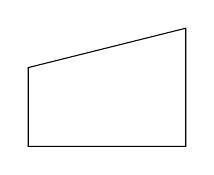
\begin{tikzpicture}
\draw (0,0) -- (2,0) -- (2,1.5) -- (0,1) -- cycle;
\end{tikzpicture}
}\quad
\subfigure[chap8fig:3][A \Bold{concave} quadrilateral.]{
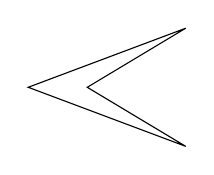
\begin{tikzpicture}[yscale=0.75]
\draw (0,1) -- (2,0) -- (0.75,1) -- (2,2) -- cycle;
\end{tikzpicture}
}\quad
\subfigure[chap8fig:4][A parallelogram.]{
\begin{tikzpicture}
\node [trapezium,trapezium left angle=60, trapezium right angle=120,minimum height=1cm,minimum width=3cm,draw] {};
\end{tikzpicture}
}\\
\subfigure[chap8fig:5][A trapezoid.]{
\begin{tikzpicture}
\node [trapezium,trapezium left angle=60, trapezium right angle=80,minimum height=1cm,minimum width=3cm,draw] {};
\end{tikzpicture}
}\quad
\subfigure[chap8fig:6][An isosceles trapezoid.]{
\begin{tikzpicture}
\node [trapezium,minimum height=1cm,minimum width=3cm,draw] {};
\end{tikzpicture}
}\quad
\subfigure[chap8fig:7][A rhombus.]{
\begin{tikzpicture}
\node [trapezium,trapezium left angle=60, trapezium right angle=120,minimum height=1.5cm,minimum width=1.5cm,draw] {};
\end{tikzpicture}
}\\
\subfigure[chap8fig:8][A rectangle.]{
\begin{tikzpicture}
\node [rectangle,minimum height=1.5cm,minimum width=2.5cm,draw] {};
\end{tikzpicture}
}\quad
\subfigure[chap8fig:9][A square.]{
\begin{tikzpicture}
\node [rectangle,minimum height=1.5cm,minimum width=1.5cm,draw] {};
\end{tikzpicture}
}\quad 
\subfigure[chap8fig:10][A kite.]{
\begin{tikzpicture}
\node [kite,kite upper vertex angle=60,kite lower vertex angle=120,minimum width=1.5cm,draw] {};
\end{tikzpicture}
}
\caption{Examples of parallelograms.}
\label{chap8fig:1}
\end{figure}

\begin{figure}[!h]
\centering
\caption{Concept Diagram for Quadrilaterals}
\begin{tikzpicture}
\node (quadrilateral) at (0,0) {};
\draw (quadrilateral)-- +(1.5,0) -- +(1.5,1.175) -- +(0,.67) -- cycle;
\node (B) [below] at ($(quadrilateral)+(1,0)$) {Quadrilateral};
\node (kite) [below left=of B,kite,kite upper vertex angle=120,kite lower vertex angle=60,minimum width=1cm,draw,label=below:kite] {};
\node (parallelogram) [below=of B,trapezium,trapezium left angle=60, trapezium right angle=120,minimum height=0.5cm,minimum width=1.5cm,draw,label=below:parallelogram] {};
\node (trapezoid) [below right=of B,trapezium,trapezium left angle=60, trapezium right angle=80,minimum height=0.5cm,minimum width=1.5cm,draw,label=below:trapezoid] {};
\node (rhombus) [below left=of parallelogram,kite,kite upper vertex angle=60,kite lower vertex angle=60,minimum height=1cm,draw,label=below:rhombus] {};
\node (rectangle) [below right=of parallelogram,rectangle,minimum height=.5cm,minimum width=1.25cm,draw,label=below:rectangle] {};
\node (isosceles trapezoid) [below right=of trapezoid,trapezium,minimum height=.5cm,minimum width=1.5cm,draw,label=below:isosceles trapezoid] {};
\node (square) [below right= of rhombus,rectangle,minimum height=1cm,minimum width=1cm,draw,label=below:square] {};
\begin{pgfonlayer}{background}
\draw ($(quadrilateral)!.5!(0,.67)$) -| (kite);
\draw (1.5,0.33) -| (trapezoid);
\draw (B) -- (parallelogram);
\draw (kite) -- (rhombus);
\draw (parallelogram) -- (rhombus);
\draw (parallelogram) -- (rectangle);
\draw (rhombus) -- (square);
\draw (rectangle) -- (square);
\draw (trapezoid.south) --  (isosceles trapezoid);
\end{pgfonlayer}
\end{tikzpicture}
\label{chap8fig:2}
\end{figure}

Additional Questions:
\begin{enumerate}
\item When can a rectangle be a square?
\item Can a rectangle be a rhombus? How?
\item Can a kite be a rhombus? How?
\end{enumerate}
Answers:
\begin{enumerate}
\item A rectangle can be a square if all the sides of the rectangle are congruent.
\item If a rectangle is a square, then it automatically becomes a rhombus.
\item A kite can become a rhombus if the two pairs of congruent sides are congruent
to one another.
\end{enumerate}
\section*{DISCUSSION}
After Activity 1 has been implemented and discussed, the participants will now examine what
happened during the activity itself. Each step of the activity will be examined for their reaction
or behavior.
\subsection*{Questions for Discussion}
\begin{enumerate}
\item After the envelopes were distributed, what did the members do? How did they behave?
Were they excited, happy, anxious, or indifferent?
\item When you were asked to classify the figures, what was the first thing that came to your
mind? What were the initial questions raised during the discussion?
\item Did everyone participate or contribute in doing the activity? What were the difficulties
encountered by the group? How did you overcome these difficulties?
\item What was the role of the teacher during the entire activity?
\end{enumerate}
In Activity 1, the teacher did not directly lecture on the topic to be discussed but
instead, the participants were given an activity to discover the relationship between the
figures given. Participants were doing more of the learning through the manipulatives and
the guide questions given by the teacher.

This type of activity is an example of an inquiry-based approach of learning.

\subsection*{What is Inquiry-Based Learning?}

As defined by the Brigham Young University’s Center for Teaching and Learning, Inquiry-
Based Learning is

\begin{Quote}
“an inductive teaching methodology that centers around students focusing on
questions and/or research (Spronken-Smith et al., 2008). Teachers engage
students by allowing them to facilitate their own learning with support and
may allow students to create their own learning situations (Spronken-Smith et
al., 2008; Feletti, 1993). “Inquiry learning” was founded around the scientific
method while “inquiry-based learning” was developed as a flexible alternative
to problem-based learning (Feletti, 1993).”
\end{Quote}
Inquiry-based learning is a teaching strategy which involves the learner more than the
traditional way of teaching. In this strategy, learners are guided to understand the concepts.
Dictionary defines inquiry as seeking knowledge, information, or truth through questioning.
Inquiry-based learning is not just asking questions, but it is a way of converting data and
information into useful knowledge. A useful application of inquiry-based learning involves many
different factors, which are, a different level of questions, a focus for questions, a framework for
questions, and a context for questions.

\subsection*{What are the types of questions?}
\begin{definition}[Types of questions in IBL]
\begin{enumerate}
\item \Bold{Inference questions}
	\begin{itemize}
	\item Mainly asked by students who want to gain extra knowledge about a
	particular topic
	\item Students can be encouraged by finding clues, examining them, and
	discussing them to justify the inferences of the topic
	\end{itemize}
\item \Bold{Interpretation questions}
	\begin{itemize}
	\item Mainly force the students to understand the consequences of the ideas
	or information
	\end{itemize}
\item \Bold{Transfer questions}
	\begin{itemize}
	\item Make students take their information to a new place, level or stage
	\end{itemize}
\item \Bold{Hypothesis questions}
	\begin{itemize}
	\item Mainly based on what can be predicted or tested through thinking
	\end{itemize}
\end{enumerate}
\end{definition}
\subsection*{What are the key principles for Inquiry-Based Learning?}
\begin{definition}[Key Principles for IBL]
\begin{enumerate}
\item \textbf{Principle 1:} All learning activities should focus on using information-processing skills (from observations to synthesis) and applying the discipline "ground rules" as a means to learn content set in a
broad conceptual context.
\item \textbf{Principle 2:} Inquiry learning puts the learner at the center of an active learning process, and the systemic
elements (the teacher, instructional resources, technology, and so forth) are prepared or aligned to support the learner.
\item \textbf{Principle 3:} The role of the teacher becomes one of facilitating the learning process. The teacher also becomes a learner by finding out more about the learner and the process of inquiry learning.
\item \textbf{Principle 4:} What is assessed is what is valued. Therefore, more emphasis needs to be placed on assessing the development of information-processing skills, nurtured habits of mind, or "ground rules" of
the discipline, and conceptual understandings rather than just the content of the field.
\end{enumerate}
\end{definition}
Inquiry-Based Learning generally follows the basic inquiry process as shown in Figure \eqref{chap8fig:3}.
There are five key elements in inquiry learning--Ask, Investigate, Create, Discuss and Reflect.
\begin{figure}[!h]
\centering
\smartdiagramset{module shape=ellipse}
\smartdiagram[circular diagram]{Ask, Investigate, Create, Discuss, Reflect}
\caption[Basic Inquiry Process]{The \Bold{Basic Inquiry Process}. Based on: \url{http://www.cii.illinois.edu/InquiryPage/inquiry/process.html}}
\label{chap8fig:3}
\end{figure}
\begin{description}
\item[Ask] It begins with the desire to discover. Meaningful questions are inspired
by genuine curiosity about real-world experiences. A question or a
problem comes into focus at this stage, and the learner begins to define
or describe what it is.

Some real examples of questions in this stage of the process are:
	\begin{itemize}
	\item "What makes a poem poetry?"
	\item "Where do chickens come from and how does an egg 'work'?"
	\item "Why does the moon change shape?"
	\end{itemize}
Of course, questions are redefined throughout the learning process. We
never fully leave one stage and go neatly to the next. As one teacher at a
recent Inquiry Workshop pointed out, "It's messy, but it works!"
Questions naturally lead to the next stage in the process: Investigation.
\item[Investigate] Taking the curious impulse and putting it into action is what we call the
investigation process. At this stage the learner begins to gather
information: researching resources, studying, crafting an experiment,
observing, or interviewing, to name a few. The learner may recast the
question, refine a line of query, or plunge down a new path that the
original question did not or could not anticipate. The information-
gathering stage becomes a self-motivated process that is wholly owned
by the engaged learner.
\item[Create] As the information gathered in the investigation stage begins to
coalesce, the learner begins to make connections. The ability at this
stage to synthesize meaning is the creative spark that forms all new
knowledge. The learner now undertakes the creative task of shaping
significant new thoughts, ideas, and theories outside of his/her prior
experience.
\item[Discuss] At this point in the circle of inquiry, learners share their new ideas with
others. The learner begins to ask others about their own experiences
and investigations. Shared knowledge is a community-building process,
and the meaning of their investigation begins to take on greater
relevance in the context of the learner's society. Comparing notes,
discussing conclusions, and sharing experiences are all examples of this
process in action.
\item[Reflect] Reflection is just that: taking the time to look back at the question, the
research path, and the conclusions made. The learner steps back, takes
inventory, makes observations, and possibly makes new decisions. Has a
solution been found? Do new questions come into light? What might
those questions be?
\end{description}
What follows are other models which are accepted and used in inquiry learning.
\subsection*{Predict--Observe--Explain (POE)}
The POE strategy was developed by White and Gunstone (1992) to uncover individual students'
predictions, and their reasons for making these, about a specific event.
\subsubsection*{When to Use}
POE is a strategy often used in science. It works best with demonstrations that allow immediate
observations, and suits Physical and Material World contexts. A similar strategy also works well in
mathematics, particularly in statistics.
\begin{itemize}
\item It can be used for finding out students' initial ideas;
\item providing teachers with information about students' thinking;
\item generating discussion;
\item motivating students to want to explore the concept; and
\item generating investigations.
\end{itemize}
\subsubsection*{The Theory}
Constructivist theories of learning consider that students’ existing understandings should be
considered when developing teaching and learning programmes. Events that surprise create
conditions where students may be ready to start re-examining their personal theories.
\subsubsection*{How the Strategy Works}
\begin{itemize}
\item Unless students are asked to predict first what will happen, they may not observe
carefully.
\item Writing down their prediction motivates them to want to know the answer.
\item Asking students to explain the reasons for their predictions gives the teacher indications
of their theories. This can be useful for uncovering misconceptions or developing
understandings they have. It can provide information for making decisions about the
subsequent learning.
\item Explaining and evaluating their predictions and listening to others' predictions helps
students to begin evaluating their own learning and constructing new meanings.
\end{itemize}
\subsubsection*{What to Do}
\begin{itemize}
\item Set up a demonstration of an event, related to the focus topic, that may surprise students,
and which can be observed.
\item Tell the students what you are going to be doing.
\end{itemize}
\paragraph*{Step 1: Predict}
\begin{itemize}
\item Ask the students to independently write their prediction of what will happen.
\item Ask them what they think they will see and why they think this.
\end{itemize}
\paragraph*{Step 2: Observe}
\begin{itemize}
\item Carry out the demonstration.
\item Allow time to focus on observation.
\item Ask students to write down what they observe.
\end{itemize}
\paragraph*{Step 3: Explain}
\begin{itemize}
\item Ask students to amend or add to their explanation to take account of the observation.
\item After students have committed their explanations to paper, discuss their ideas together
\end{itemize}
\subsection*{Problem-Based Learning}
At the University of Delaware, they use Problem-based learning in their undergraduate
courses. According to them, in a problem-based learning (PBL) model, students engage complex,
challenging problems and collaboratively work toward their resolution. PBL is about students
connecting disciplinary knowledge to real-world problems--the motivation to solve a problem
becomes the motivation to learn.

With PBL, the teacher gives the students problems to work on and not the lectures or
exercises or assignments. Content is not readily given. Instead, students should work on the
given problem to draw out the necessary concepts to be learned. The teacher acts as a
facilitator who will guide the students in solving the problems instead of being the source of
solutions.

Problem-based learning will provide the students opportunities for the following:
\begin{itemize}
\item examine and try out what they know;
\item discover what they need to learn;
\item develop their people skills for achieving higher performance in teams;
\item improve their communications skills;
\item state and defend positions with evidence and sound argument;
\item become more flexible in processing information and meeting obligations; and
\item practice skills that they will need after their education.
\end{itemize}
An example of how the students can learn through PBL is shown below using a simplified
model for PBL.
\begin{enumerate}
\item \textit{Explore the issues.} 

Your teacher introduces an "ill-structured" problem to you.
Discuss the problem statement and list its significant parts.
You may feel that you don't know enough to solve the problem but that is the
challenge!

You will have to gather information and learn new concepts, principles, or skills as you
engage in the problem-solving process.

\item \textit{List "What do we know?"} What do you know to solve the problem?
This includes both what you actually know and what strengths and capabilities each
team member has.
Consider or note everyone's input, no matter how strange it may appear: it could hold a
possibility!

\item \textit{Develop, and write out, the problem statement in your own words.} 

A problem statement should come from your/the group's analysis of what you know,
and what you will need to know to solve it. You will need:

	\begin{itemize}
	\item a written statement
	\item the agreement of your group on the statement; and
	\item feedback on this statement from your instructor.
	(This may be optional, but is a good idea.)
	
	\textit{Note:} The problem statement is often revisited and edited as new information is
	discovered, or "old" information is discarded.
	\end{itemize}
\item\label{chap8item:1} \textit{List out possible solutions.} List them all, then order them from strongest to weakest.
Choose the best one, or most likely to succeed.
\item \textit{List actions to be taken with a timeline.} 
	\begin{itemize}
	\item What do we have to know and do to solve the problem?
	\item How do we rank these possibilities?
	\item How do these relate to our list of solutions?
	Do we agree?
	\end{itemize}
\item \textit{List "What do we need to know?"}

Research the knowledge and data that will support your solution.
You will need to information to fill in missing gaps.
	\begin{itemize}
	\item Discuss possible resources, such as experts, books, web sites, etc.
	\item Assign and schedule research tasks, and their corresponding deadlines.
	\end{itemize}
If your research supports your solution, and if there is general agreement, go to item \eqref{chap8item:2}.
If not, go back to item \eqref{chap8item:1}.

\item \label{chap8item:2}\textit{Write up your solution with its supporting documentation, and submit it.} You may need to present your findings and/or recommendations to a group or your
classmates. This should include the problem statement, questions, data gathered, analysis of data, and
support for solutions or recommendations based on the data analysis, in short, the process
and outcome.

\item \textit{Present and defend your conclusions.} The goal is to present not only your conclusions, but the foundation upon which they
rest. Prepare to:
	\begin{itemize}
	\item state clearly both the problem and your conclusion;
	\item summarize the process you used, options considered, and difficulties encountered;
	\item convince, not overpower;
	(Bring others to your side, or to consider without prejudice your supporting
	documentation and reason.)
	\item help others learn, as you have learned; and
	\item if challenged and you have an answer, present it clearly.
	(If you don't have an answer, acknowledge it and refer it for more consideration.)
	\end{itemize}
\end{enumerate}
\subsection*{5E Instructional Model}
The 5E's instructional model provides a format for lessons that
builds on what students already know. The 5E's sequence the
learning experience so that learners construct their
understanding of a concept across time. Each phase of the
learning sequence can be described using five words that begin
with "E": Engage, Explore, Explain, Extend, and Evaluate.
\begin{figure}[!h]
\centering
\includegraphics[width=0.3\linewidth]{5E}
\caption[The 5E Instructional Model]{Source: \fullcite{5eim}}
\label{chap8fig:4}
\end{figure}
\begin{longtable}{@{}>{\bfseries\arraybackslash}lp{0.3\linewidth}p{0.3\linewidth}@{}}
\kill
\caption{Sequences of the 5E Instructional Model\label{chap8tab:1}}\\
\hline \hline
\textbf{Learning Phase} & \textbf{Student Rule} & \textbf{Teacher Rule}\\
\hline \hline
\endfirsthead
\caption[]{(continued)}\\
\hline \hline 
\textbf{Learning Phase} & \textbf{Student Rule} & \textbf{Teacher Rule}\\
\hline \hline
\endhead
\hline \hline 
\multicolumn{3}{l}{Continued to next page}\\
\hline
\endfoot
\endlastfoot
Engage/Excite & Students are introduced to the concept. 
Students make connections to prior 
knowledge and what is to be studied. 
Student thinking is clarified. Students 
become mentally engaged in the new 
learning experience. &
Teachers ask questions of
students and engage them in the
guided inquiry lessons. They use
strategies that make connections
between the past and present
learning experience. Teachers set
a level of anticipation.\\
Explore & Students explore or experiment at this point. 
They engage in observations, use science 
tools and materials (manipulatives), collect 
data, and record data. &
Teachers set up the investigation
and guide students in inquiry,
asking probing questions to clarify
understanding.\\
Explain & Students verbalize their understandings from 
the "explore" phase, look for patterns in 
their data, and describe what they observed. 
This can be done in small and/or whole 
groups. & 
Teachers ask probing questions
that encourage students to look
for patterns or irregularities in
their data.\\
Elaborate & Students expand their learning, practice skills 
and behavior, and make connections or 
applications to related concepts and in the 
world around them. & Teachers provide learning
opportunities for students to
apply their knowledge and to gain
a deeper understanding. Activities
can include reading articles and
books, writing, designing other
experiments, and exploring
related topics on the Internet. \\
Evaluate & Students answer questions, pose questions, 
and illustrate their knowledge 
(understandings) and skills (abilities). & 
Teachers diagnose student
understanding through an
ongoing process. Assessment can
be both formative (ongoing and
dynamic) and summative (end-of-
lesson final test or product).\\
\hline
\end{longtable}
\newpage
\subsection*{7E Instructional Model}
The 7E Instructional model is based on the 5E model but expands the engagement
phase to elicit and engage. The elaborate and evaluate phases are expanded to elaborate,
evaluate and extend, as well. The purpose of the 7E model is to emphasize the importance of
recognizing prior knowledge and expanding knowledge gained through conceptual change
(Eisenkraft, 2003). % No Eisenkraft in References.

\begin{figure}[!h]
\centering
\includegraphics[width=\linewidth]{7E}
\caption[The 7E Instructional Model Used in Active Chemistry]{Source: \fullcite{7eim}}
\label{chap8fig:5}
\end{figure}
These instructional elements will help to structure lessons to be Inquiry based.
\begin{longtable}{@{}>{\bfseries\arraybackslash}lp{0.4\linewidth}@{}}
\kill
\caption{Instructional Elements of the 7E Instructional Model\label{chap8tab:2}}\\
\hline \hline
\endfirsthead
\hline \hline 
\endhead
\hline \hline 
\multicolumn{2}{l}{Continued to next page}\\
\hline
\endfoot
\endlastfoot
Elicit & Identify what students know.\\
Engage & Creates interest
students.\\
Explore & Provides activities and experiments for students to
collect and analyse data\\
Explain & Encourage students to explain concepts followed by
formal explanation by teacher.\\
Elaborate & Provide opportunity for students to apply
knowledge and skills learnt in new but similar
situations.\\
Evaluate & Assess understanding and abilities of the students.\\
Extend & Students try to apply new knowledge and skills in
completely unfamiliar situations.\\
\hline
\end{longtable}
\subsection*{4E $\times$ 2 Instructional Model}
The 4E $\times$ 2 Instructional Model
was designed to unite three major
learning constructs (inquiry instruction,
formative assessment, and reflective
practice) that have all been shown to
improve learning. When well integrated
these learning constructs help facilitate
deeper teaching and more powerful
learning experiences. All the lessons
designed and available under the lesson
plan tab use the 4E $\times$ 2 Model.
\begin{figure}[!h]
\centering
\includegraphics[width=0.5\linewidth]{4ex2}
\caption[$4\mathrm{E}\times 2$ Instructional Model]{\Bold{4E $\times 2$ Instructional Model}. Source: \fullcite{marshall}}
\label{chap8fig:6}
\end{figure}
\subsection*{GROUP ACTIVITY 2}
The participants will again be grouped into 5 or 6. The groupings in the morning may be
retained for this activity.

Each group must come up with their own inquiry-based activity or lesson plan. Each group can
choose one topic among the following to work on. Outputs shall be written on the Manila Paper.

\begin{center}
\begin{tabular}{p{0.3\linewidth}p{0.3\linewidth}}
\hline 
Points, Lines and Planes & Subsets of a Line\\
Different Kinds of Angles & Angle Pairs\\
Vertical Angles and Angles formed by Transversals & Classification of Triangles\\
Relationship of Sides and Angles in Triangles & Convex Polygons\\
Quadrilaterals & Exterior and Interior Angles of Convex Polygons\\
Circles & \\
\hline 
\end{tabular}
\end{center}
\subsection*{SAMPLE ACTIVITIES, LESSON PLAN and LESSON PLAN TEMPLATES}
\begin{itemize}
\item Sum of Interior Angles: \fullcite{sia}
\item Geometry and the Real World: \fullcite{abdul}
\item 5E Lesson Plan: The Geometry for Pentominoes: \fullcite{uoh}
\end{itemize}
After the workshop, each group will present their output to the body for critiquing
and suggestions.
\subsection*{How to Evaluate Inquiry-based Instruction}
The Electronic Quality of Inquiry Protocol (EQUIP) instrument is designed to measure
the quantity and quality of inquiry instruction being facilitated in K-12 math and science
classrooms. The instrument does not seek to measure all forms of quality instruction–only those
that are inquiry-based in nature. \textcite{4e2} provides a form which can be used for peer
evaluation and classroom observations.

Included in this file are four rubrics to evaluate instructional, discourse, assessment, and
curriculum factors. For each construct measured, the evaluator will determine if the implementation of the lesson plan is at pre-inquiry (level 1), developing inquiry (level 2),
proficient inquiry (level 3) or exemplary inquiry (level 4). Pre-inquiry level suggests that it is
more teacher-centered rather than student centered while a rating of 4 would indicate more
student participation in acquiring learning.